%%% detailed description of the protocols, software and algorithms used for the project
\chapter{Materials and methods} % at least 3 pages, maximum 10 pages

%%%%%%%%%%%%%%%%%%%%%%%%%%%%%%%%%%%%%%%%%%%%%%%%%%%%%%%%%%%%%%%%%%%%%%%%%%%%%%%%
\section{Computational environments}
  All the calculations and data handling required for the modelling and potential calculations were performed using \textbf{Python} version 3.10.5 \cite{python_2009}. Even if it is not the most performant option, its flexibility and seamless syntaxis allow for quick experimentation when developing the models; it is well known for its powerful data visualization packages, such as \textbf{Matplotlib} \cite{python_2021}. Nevertheless, the performance of the calculations was optimized by employing the package \textbf{NumPy} for parallelizable matrix computations \cite{numpy_2020}, \textbf{pandas} for data manipulation \cite{pandas_2020} and multiprocessing techniques from the standard library.

  Furthermore, for parsing PDB files, the Python package \textbf{MDAnalysis} (MDA) is used \cite{mda_2016, mda_2011}. This package allows for selecting specific atoms of the system by means of a query, which is useful for performing operations using only the atoms of interest. Matrices with values for the potentials are stored using the \textbf{JSON} \cite{json_web} and \textbf{DX} \cite{opendx_web} specifications.

  The visualization software \textbf{VMD} \cite{vmd_96} was used as a reference points for testing with queries for molecular selections, representations and other aspects of the pipeline. All new molecular visualization and user interaction procedures where developed in \textbf{UnityMol} \cite{unitymol_web}, by employing the GUI-based development workflow provided by \textbf{Unity3D}. Necessary scripts were written using the language \textbf{C\#}, as required by the engine \cite{unity_2014}.


%%%%%%%%%%%%%%%%%%%%%%%%%%%%%%%%%%%%%%%%%%%%%%%%%%%%%%%%%%%%%%%%%%%%%%%%%%%%%%%%
\section{Characterization of Physicochemical Properties}
  \subsection{Model Conditions}
    Standard visualization techniques involve at most four dimensions in a single time frame, namely three spatial dimensions and color/opacity. Time can be added as a fifth dimension, either by employing animations or interactive sliders. However, depending on the data, this can impact ergononomity and intuitiveness, as information can not be visualized all at once in a single time frame. Therefore, the combined amount of dimensions used by the domain (i.e. "input") and codomain (i.e. "outputs") of the potential models was fixed to maximum four.

    The physicochemical properties were modelled either by means of a \textit{physical energy function} (in the case of electrostatics) or a \textit{statistical energy function} (in the case of stacking, hydrogen bonds and hydrophobicity). In both cases, the domain of the functions consisted of the three spatial dimensions of the molecular systems. This means that the codomain of the functions was limited to only one dimension, i.e. only one output. For the \textit{physical energy function}, this output corresponds to the respective physical value at each spatial coordinate, while for the \textit{statistical energy functions} the output corresponds to a propensity value of how likely an atom or group is to be at each spatial coordinate.

  \subsection{Stacking Potential}
    \subsubsection{Obtaining the Datasets}
      For modeling the stacking potential, the shape and parameters of a statistical energy function were empirically determined. A large dataset of protein, protein/ligand, protein/nucleic and protein/nucleic/ligand systems was downloaded from the Protein Data Bank (PDB) \cite{pdb_2003}. First of all, the PDB ids for these systems were obtained by submitting two queries to the database:

      \begin{itemize}
        \item \textbf{For protein and protein/ligand}: \textcolor{teal}{"entry polymer types = protein only" \& "number of assemblies = 1" \& "experimental method = X-ray diffraction" \& "data collection resolution < 2.5 \AA"}
        \item \textbf{For protein/nucleic and protein/nucleic/ligand}: \textcolor{teal}{"entry polymer types = protein/NA" \& "number of assemblies = 1" \& "experimental method = X-ray diffraction" \& "data collection resolution < 2.5 \AA"}
      \end{itemize}

      These PDB ids were used to programatically download the dataset by means of bash scripts and interacting with the PDB's API. Then, a Python script was employed for extracting ligand names from the PDB files. These names were similarly used for downloading a dataset of CIF ligand description files from PDB.

    \subsubsection{Detecting Aromatic Groups in Ligands}
      For parametrizing this model, only ligands with aromatic groups are of interest. A first approach for filtering the ligands was to parse the SMILES string from the CIF files and keep only those that contained flags for presence of aromatic bonds (i.e. lowercase letters).

      After some issues with the first method, a second approach was also deviced. A Python script was used for inspecting the bonds topology described in the CIF files. A ligand was considered to be candidate for aromaticity if its structure had cycles after discarding tetrahedral atoms (i.e. those with four bonds). In this case, information about the individually detected cycles was stored in a CSV file.

      Ligands where the two methods coincided were considered to have an aromatic group for the next steps. Cases where the methods disagreed were manually inspected to decide whether to consider them aromatic or not.

    \subsubsection{Coarse-grained Description of Aromatic Groups}
      Before sampling the aromatic interactions, all aromatic groups are simplified into a coarse-grained description. For each aromatic group, a particle is defined at the \textbf{center of geometry} (COG) of the group (i.e. the average position of the atoms that conform it). In cases where an aromatic group is made by two adjacent aromatic rings (such as tryptophan or adenine), the center of geometry of the whole group is considered as a single point. The \textbf{normal vector} of the aromatic plane (i.e. the three-dimensional vector perpendicular to the plane) is also calculated for each group (figure \ref{fig:methods/aromatic}).

      \begin{figure}[H]
        \centering
        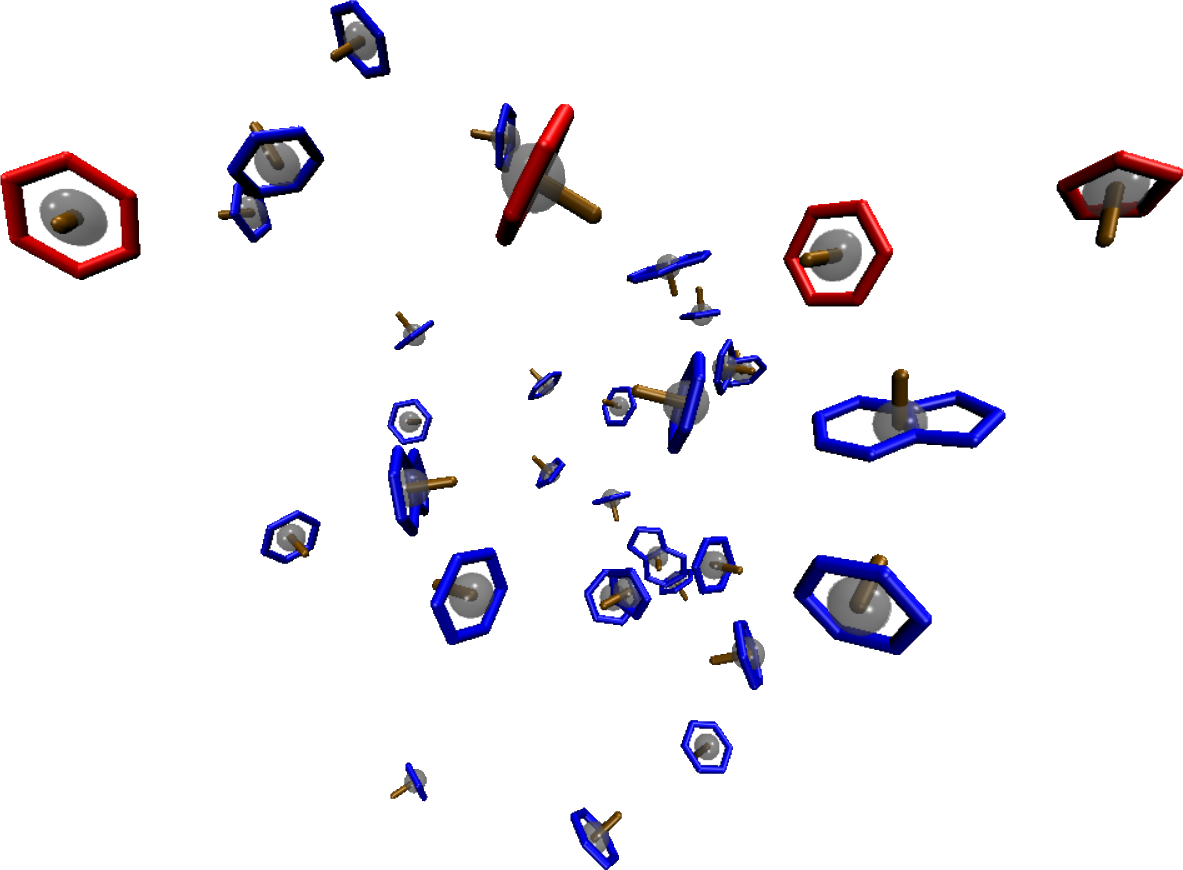
\includegraphics[width=0.5\textwidth]{figures/methods/aromatic.png}
        \caption{\label{fig:methods/aromatic} Aromatic groups and their coarse grained representation. Blue) aminoacid aromatic rings, Red) nucleic acid aromatic rings, Silver) center of geometry, Bronze) normal vector. PDB: 1IQJ. Rendered in VMD.}
      \end{figure}

      Atoms corresponding to aromatic groups are selected by a query that specifies the aromatic residue names and the specific atom names that compose their aromatic rings. This information is stored in lookup tables, which are straightforward in the case of amino and nucleic acids, although \textit{synonyms} must be covered (i.e. a residue having more than one possible name, such as adenine been identified as \textbf{A} or \textbf{ADE} in different PDB files).

      Additionally, some synonyms used by MDA for amino or nucleic acids are actually used by PDB for unrelated ligands (for example \textbf{THY} refers to thymine according to MDA but to a ligand according to PDB). This ligand information is stored in the look up tables just for good measure. Finally, the look up table for the ligands is simply the curated CSV file obtained from the ligand dataset in the previous step. Note that, whenever a ligand has more than one separate aromatic group in their structure, each group is reported as a separate row. The lookup tables employed for protein (table \ref{tab:methods/aromatic_prot}), nucleic (table \ref{tab:methods/aromatic_nucleic}) and the first twenty rows for ligands (table \ref{tab:methods/aromatic_ligand}) are available at Appendix I.

    \subsubsection{Sampling of Aromatic Interactions}
      Two aromatic groups were considered to interact when their corresponding coarse-grained particles where under a certain distance range, set to be between {3 \AA} and {6.5 \AA} following the observations of similar data analysis studies \cite{aromatic_2018}. To obtain all aromatic interactions present in a PDB file, an all-to-all pairwise confrontation was done between the aromatic groups of the system. For those under the spatial proximity of interest, the distance and the $\alpha$ and $\beta$ angles were calculated.

      Note that, given two particles $i$ and $j$, the distance and $\beta$ values are the same for the $i-j$ and $j-i$ interactions, however the $\alpha$ values my differ between $i-j$ and $j-i$. Therefore, for each pair of aromatic groups, two interaction datapoints are produced, with duplicate distance and $\beta$ values and possibly unique $\alpha$ values. This process was performed over the entire dataset of PDB files, employing multithreading to speed up the process.

    \subsubsection{Model Definition}
      After filling the interactions dataframe, standard data visualization techniques were performed to observe how the distance, $\alpha$ and $\beta$ values interacted. Observing the histograms obtained from these data allowed for extracting an empirical shape and parameters for the distribution of stacking interactions, needed for defining the stacking potential model. This consisted of a \textbf{sum of probability distributions}, with said empirically defined shape and centered in the COG of each aromatic group.

  \subsection{Hydrogen Bonds Potential}
    Theoretically, modeling hydrogen bond interactions depends on the distances and angle between acceptor, donor and the hydrogen atom. However, when generating a statistical potential field, only acceptor or donor+hydrogen are available, as by definition the potential field is built to estimate the most probable configurations for the missing second half of the interaction. This means that, if the potential field is built without introducing simplifications, the domain of the function would consist of four dimensions (three spatial dimensions plus the \textit{hydrogen bond angle} dimension) to properly describe the interaction, exceeding the maximum defined previously.

    Therefore, for modeling the hydrogen bond interactions, an assumption is made that only hydrogen bonds with an ideal angle of approximately $180^{\circ}$ are considered. The model is further simplified by neglecting the position of any hydrogen atoms in the PDB structure, based in the idea that usually the positions of the hydrogen atoms vary much fast than that of the donor atoms, which means it is better to base the model only on where the donors and acceptors might be.

    With this in mind, the hydrogen bond potential model was defined as a \textbf{sum of univariate normal distributions} centered in the acceptor and donor atoms of the structure of interest. The only parameter considered by the model was the distance from any given acceptor or donor atom to any point in the three-dimensional space. The parameters for the probability distribution are $\mu = 3$ and $\sigma = 0.15$ [TODO: cite?].

  \subsection{Electrostatic Potential}
    Quantifying the electrostatic potential around atoms of a molecular system overlaps smoothly with the functionality of the APBS software. Hence, there is no need to model the interaction potential in this case and it is enough to incorporate the APBS pipeline into the workflow. However, there might be issues in the visualization stage with the fact that this potentials can vary significantly in magnitude (figure \ref{fig:methods/lapbs}.0).

    \begin{figure}[H]
      \centering
      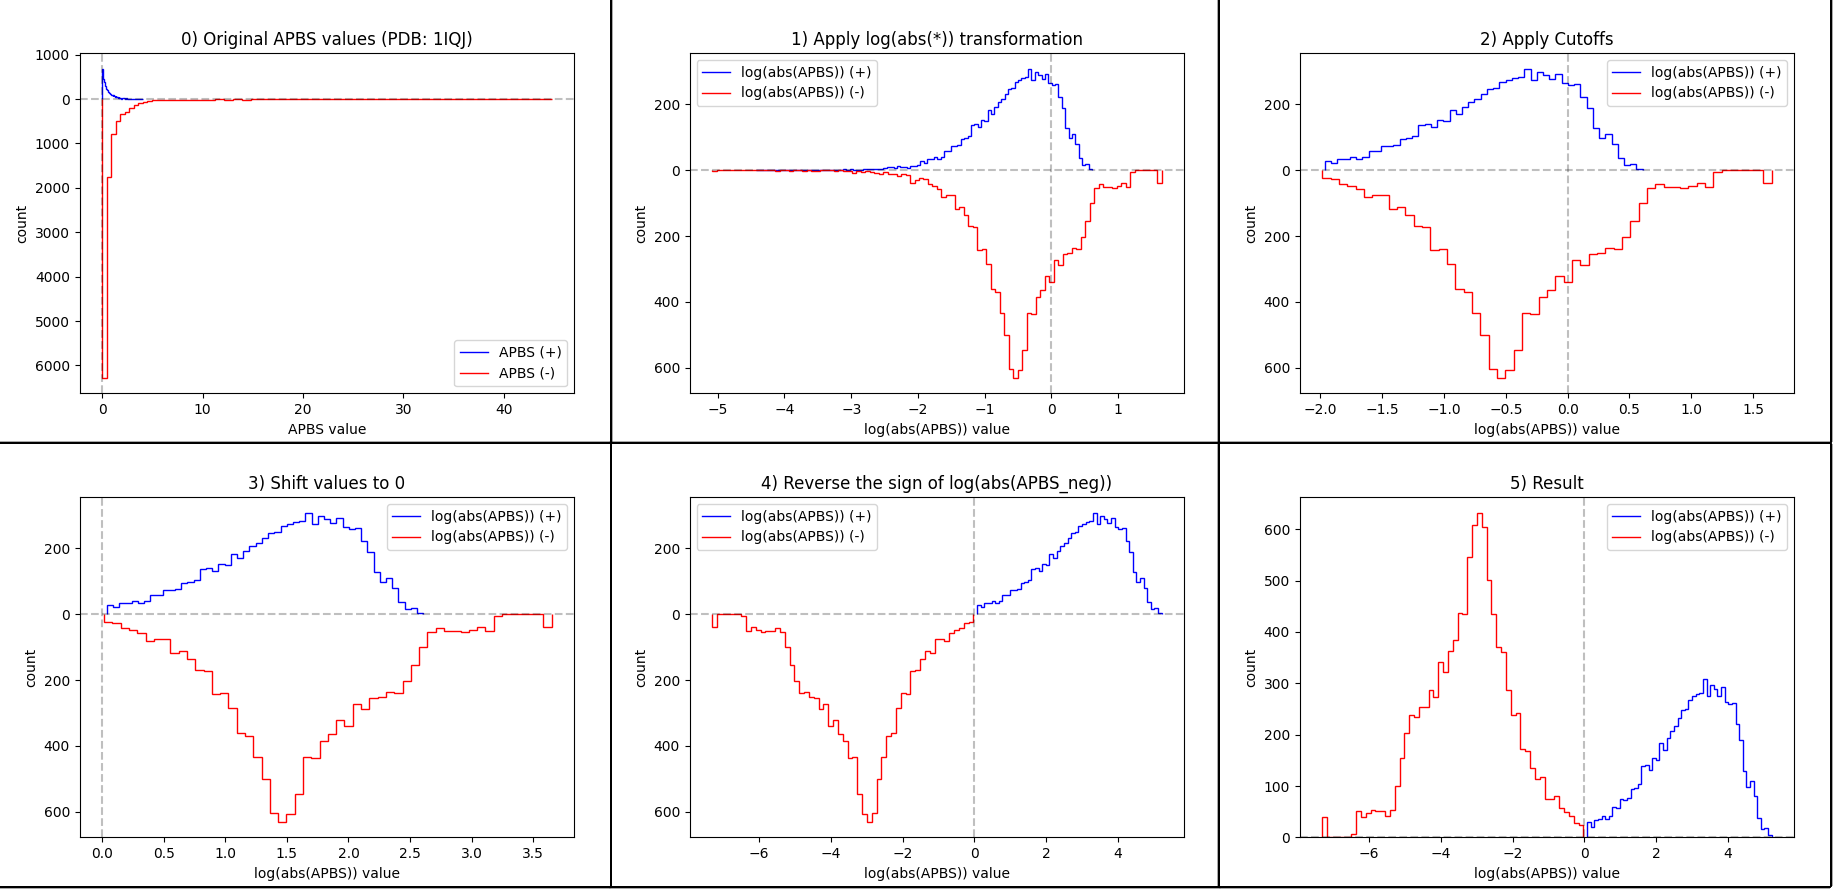
\includegraphics[width=1\textwidth]{figures/methods/lapbs.png}
      \caption{\label{fig:methods/lapbs} [TODO: description, transpose image source? (2x3 layout instead of 3x2). change labels to alphabetical]}
    \end{figure}

    Although moving the values into the logarithmic scale is the intuitive solution for this problem, it can not be done in a straightforward way, as the model  calculates actual physical values related to the charges of the system (instead of propensity values as in the previous cases) which can also be negative. To avoid negative values, the absolute value of the points is taken before applying the logarithm base 10 (figure \ref{fig:methods/lapbs}.1).

    By applying this transformation, negative and positive values are obtained, which this time represent the \textit{scale} of the quantities instead of their \textit{physical} meaning; it is evident however that both are important to conserve. To achieve this, the transformed set of points is first pruned to conserve only meaningful and common values. This is done by applying two empirical cutoffs: a minimum of $-2$ and a maximum of $3$ (figure \ref{fig:methods/lapbs}.2) This procedure fixes the boundaries for the points, which in turn allows to shift their origin to 0 by substracting the value of the lower boundary (figure \ref{fig:methods/lapbs}.3).

    Now that all points are positive and the scale information is still conserved, it is time to bring back the physical meaning of signed electrostatic potential. To achieve this, the points that originally corresponded to negative APBS values are simply multiplied by $-1$ to reverse their sign (figure \ref{fig:methods/lapbs}.4). In this step, all points are also scaled by a factor of $2$, with the purpose of having the boundaries at a fixed $[-10, 10]$ range, and the points neatly normalized in between (figure \ref{fig:methods/lapbs}.5).

  \subsection{Hydrophobicity Potential}
    The hydrophobicity potential was modelled in a similar way to the hydrogen bonds, as a sum of univariate normal distributions centered around every atom of interest. The parameters for the probability distribution are $\mu = 3.7$ and $\sigma = 0.15$ [TODO: cite?]. Each distribution is scaled by a hydrophobicity value, which depends on the type of residue from which the atom is part of. For aminoacids, these values correspond to the Kyte-Doolittle scale, which uses positive values to represent hydrophobic residues and negative values for hydrophilic. On the other hand, this model was not implemented for RNAs, due to their mostly hydrophilic nature.


%%%%%%%%%%%%%%%%%%%%%%%%%%%%%%%%%%%%%%%%%%%%%%%%%%%%%%%%%%%%%%%%%%%%%%%%%%%%%%%%
\section{Development of Visualization Methods}
  \subsection{Graphical User Interface}
    A menu component was built for the Graphical User Interface (GUI) of UnityMol, to allow for an easy interaction between the user and the potentials calculation and visualization, from now on referred to as the \textbf{PSMenu}. The user is expected to load a PDB file and select a set of atoms related to a binding pocket (this would be usually a ligand already present in the system), using the standard UnityMol GUI. The user then can interact with a first instance of the PSMenu (figure \ref{fig:methods/umol_ps-start}), by providing the name of the atom selection and whether the system of interest is RNA based or not (defaults to protein based).

    \begin{figure}[H]
      \centering
      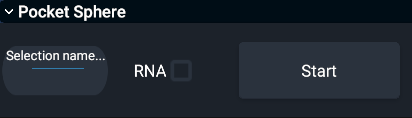
\includegraphics[width=0.5\textwidth]{figures/methods/umol_ps-start.png}
      \caption{\label{fig:methods/umol_ps-start} First instance of the PSMenu. It serves as an entry point for the visualization pipeline.}
    \end{figure}

    Once the user clicks the \textit{Start} button, a series of changes occur. First, the atoms from the user provide selection are taken as a reference to estimate the pocket position and dimensions. The pocket is approximated as a sphere, whose diameter corresponds to the distance between the two farthest atoms of the selection, and its center is simply the point in between these two atoms. This sphere will be referred to as \textbf{PS}, short for \textit{Pocket Sphere}, and it is by default represented as a translucid sphere on top of the pocket. Then, selections for the atoms inside and outside the PS are automatically generated, useful for assigning them different representations to highlight the pocket. Finally, the PSMenu changes to allow for the main functionalities of the visualization pipeline (figure \ref{fig:methods/umol_ps-main}).

    \begin{figure}[H]
      \centering
      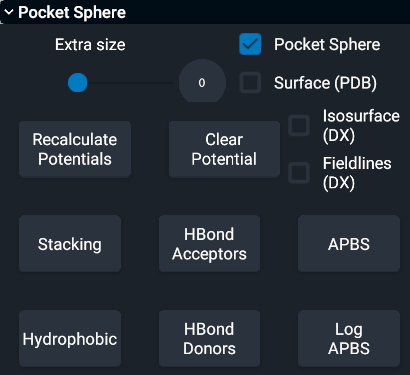
\includegraphics[width=0.5\textwidth]{figures/methods/umol_ps-main.png}
      \caption{\label{fig:methods/umol_ps-main} Main instance of the PSMenu. It gives access to the core functionalities of the visualization pipeline.}
    \end{figure}

    The size of the PS can be increased by means of the \textit{Extra size} slider, which also updates the pocket/non-pocket selections. The translucid sphere that represents the PS can be toggled on or off with the \textit{Pocket Sphere} toggle, while the cartoon-licorice based representations can be changed to surface representations with the \textit{Surface (PDB)} toggle.

    The potential fields can be calculated by clicking the \textit{Recalculate Potentials} button, although this will not display any potential by its own. THe potential field of interest can be displayed individually by clicking on its respective button, be it \textit{Stacking}, \textit{HBond Acceptors}, \textit{APBS}, \textit{Hydrophobic}, \textit{HBond Donors} or \textit{Log APBS}. The displayed potentials can be cleared from the screen by clicking on the \textit{Clear Potential} button.

    The user can switch between the two volumetric representations available for the potential fields by toggling on or off the \textit{Isosurface (DX)} toggle. The \textit{Fieldlines (DX)} toggle is not described in this work, as it is in an experimental stage and it just seeks to simplify the usage of a third volumetric representation already provided by UnityMol (i.e. fieldlines).

  \subsection{Potentials Calculation}
    \subsubsection{Populating the Potential Grids}
      Whenever the \textit{Recalculate Potentials} from figure \ref{fig:methods/umol_ps-main} button is pressed, information about the PS (such as center, diameter, path to the PDB file and whether the system corresponds to RNA) is stored into a JSON file. A Python script is then executed to proceed with the calculation pipeline. The algorithm recovers the center and diameter of the sphere from the JSON file to approximate the binding pocket of the system as a cube in the same position. This volume is then separated into small subunits of volume, regularly spaced in any given axis (although the amount of subunits may change between axes). The subunits are further discretized into points of a three-dimensional NumPy matrix.

      The matrix is filled with values for the different potentials, by employing the models described before. Atom selections are handled by MDA, while the actual numerical operations use NumPy methods to increase performance. In the case of APBS potentials, the APBS pipeline must be followed beforehand until obtaining the DX file with the results. These are then taken by the Python scripts to perform further adjustments and operations.

    \subsubsection{Trimming the Potential Grids}
      Once the potential grids are populated with values, they spatially represent a \textit{cube} of data for the potential fields. These need to be at least refined into \textit{spheres} to fit the concept of the PS pipeline, and ideally remove all other unnecesary grid points from the visualization. This process is referred to here as \textbf{trimming}, and is achieved by setting unwanted grid values to $0$. The PS pipeline employ three trimming strategies:

      \begin{itemize}
        \item \textbf{Sphere trimming}: Points whose distance from the COG is larger than the PS are set to $0$. This restricts the shape of the grid into a sphere when visualizing it.

        \item \textbf{Occupancy trimming}: Points whose position is in close proximity to pocket atoms are set to $0$, as they correspond to sections of volume already occupied by said atoms and are not plausible positions for a pharmacophore. The distance treshold for proximity is set to {3 \AA}.

        \item \textbf{RNDS trimming}: The \textit{occupancy trimming} procedure can disconnect the grid into clusters of points, corresponding to the actual pocket volume and nearby possibly unrelated cavities. To remove these cavities is performing a graph traversal strategy can be employed, starting from the COG and visiting all untrimmed neighbouring points; points that were not visited at the end of the traversal are futher trimmed out.

        In some cases, grid points corresponding to the COG can be actually trimmed by occupancy, so the starting queue is set to a small sub-cube centered around the COG, set here to have dimensions $7 \times 7 \times 7$. As the starting queue corresponds to multiple points, it is implemented as an unordered set, to avoid having duplicates in the first iterations. This also implies that points in the queue are explored in an unpredicable order, so it is referred here as a \textbf{random search} (hence the acronym \textit{RNDS}). It is worth noting that, for this particular application, the search order does not affect the final outcome of the algorithm.

        Finally, the random search was implemented so that it ignores points exceeding a \textit{search distance}, which corresponds to the length of the minimum path required to traverse from a given point to the COG sub-cube. The default value of the maximum search distance is set to infinity, effectively disabling this constraint, however it can be set to other values to further denoise the pocket volumes.

      \end{itemize}

    \subsubsection{Exporting the Potential Grids}
      Finally, each potential grid is stored twice, both as a JSON file and as a DX file. This is not only a measure to communicate the results between Python and UnityMol, but also allows for a fast display of the different grids by just loading the precomputed data files instead of performing the potential calculations every time. The DX format is also a standard way to represent grid data, so these files can be opened with other visualizers if needed.

  \subsection{Potentials Visualization}
    A first idea for how to repersent three-dimensional grids of data in an intuitive way was to generate \textit{clouds} of points, which would ideally be denser in regions where the values for the potentials are higher. This appropriately named \textbf{cloud representation} of volumetric data was implemented from scratch in UnityMol. This method normalizes the values of the potentials to assign appropriate color and opacity levels to the points.

    The precomputed JSON files are loaded by a C\# script that populates a three-dimensional array with the potential values. It then takes advantage of optimized multiprocessing routines to build the vertices and triangles of a cubic mesh, giving to each vertex a color that corresponds to its respective potential value. These meshes are then handled by a shader GPU program that assigns semi-transparent colors to the triangles according to their neighbouring vertices: more saturated and opaque colors imply higher potential values. Note that grid points whose potential values are equal to 0 are still represented by vertices and triangles in the mesh, but the shader colors them totally transparent.

    Alternatively, the potential grids can be visualized using an \textbf{isosurface representation}. In this case, the PSMenu only takes care of using the internal UnityMol APIs to open the DX file of interest and building the representation. For the potentials that require negative values (namely \textit{APBS}, \textit{LogAPBS} and \textit{Hydrophobicity}), two isosurface representations are built: one for the positive values and another for the negative ones. This allows to color them appropriately and further differentiate them by using distinct configurations of \textit{solid}, \textit{translucid} or \textit{wireframe} between the two.


%%%%%%%%%%%%%%%%%%%%%%%%%%%%%%%%%%%%%%%%%%%%%%%%%%%%%%%%%%%%%%%%%%%%%%%%%%%%%%%%
\section{Benchmarking}
  A collection of 10 protein based (table \ref{tab:methods/benchmark_prot}) and 10 RNA based (table \ref{tab:methods/benchmark_rna}) PDB files was assembled to carry out benchmarks on the potential calculations and their visualization. The protein structures were chosen from a literature review of binding pockets with different characteristics of interest. The RNA structures were obtained as a representative set of complexes from the RNA-ligand interaction database Hariboss \cite{hariboss_2022}. The potentials were calculated on the 20 systems, after removing any ligands and considering only the binding pocket of interest from the target macromolecules.

  \begin{table}[H]
    \caption{\label{tab:methods/benchmark_prot} [TODO: description].}
    \centering
    \begin{tabular}{ccccp{1.5in}p{1.5in}c}
      \hline
      PDB  & Ligand & Atoms & pKD   & Description                                & Comments                                                                   & Study                            \\ \hline
      1BG0 & ADP     & 2817  & -     & arginine kinase                            & negatively charged pocket - NO3 and Mg also participate in the active site & \cite{benchmark_negative_2000}    \\ \hline
      1EBY & BEB     & 1522  & 9.70  & HIV-1 protease in complex with inhibitor   & strong pocket affinity                                                     & \cite{benchmark_strong_2021}      \\ \hline
      1EHE & HEM     & 3100  & -     & cytochrome P450NOR                         & positively charged pocket                                                  & \cite{benchmark_positive_2001}    \\ \hline
      1H7L & TYD     & 1976  & -     & glycosyltransferase                        & -                                                                          & \cite{benchmark_1h7l_2001}        \\ \hline
      1IQJ & XMH     & 2241  & -     & serine protease - blood coagulation factor & -                                                                          & to be published                   \\ \hline
      1OFZ & FUL     & 4891  & 4.62  & fungal lectin                              & hydrogen bonds                                                             & \cite{hbonds_2023}                \\ \hline
      3DD0 & EZL     & 2074  & 9.00  & carbonic anhydrase II                      & strong pocket affinity                                                     & \cite{benchmark_strong_2021}      \\ \hline
      3EE4 & MYR     & 2320  & -     & Mn/Fe oxidase from M. tuberculosis         & hydrophobic pocket                                                         & \cite{benchmark_hydrophobic_2009} \\ \hline
      5M9W & 7GR     & 4856  & 2.24  & thermolysin in complex with inhibitor      & hydrophobic pocket                                                         & \cite{hydrophobic_2017}           \\ \hline
      6E9A & J0S     & 1705  & 11.92 & HIV-1 protease                             & strongest pocket affinity reported in PDBbind                              & \cite{pdbbind_2004}               \\ \hline
    \end{tabular}
  \end{table}

  \begin{table}[H]
    \caption{\label{tab:methods/benchmark_rna} [TODO: description]. All structures are taken from Hariboss \cite{hariboss_2022}.}
    \centering
    \begin{tabular}{ccccp{1.5in}p{1.5in}}
      \hline
      PDB  & Ligand & Atoms & pKD  & Description                                                 & Comments                                                \\ \hline
      1AKX & ARG     & 965   & -    & HIV-2 trans activating region RNA complex with argininamide & confusing for APBS pipeline - takes ligand as a protein \\ \hline
      1I9V & NMY     & 1632  & 3.47 & phenylalanine transfer RNA                                  & -                                                       \\ \hline
      2ESJ & LIV     & 900   & -    & 16S-rRNA A site                                             & -                                                       \\ \hline
      4F8U & SIS     & 922   & -    & ribosomal decoding site                                     & -                                                       \\ \hline
      5BJO & 747     & 1568  & -    & corn RNA aptamer in complex with DFHO                       & large SiteScore (1.090) on Hariboss                     \\ \hline
      5KX9 & 6YG     & 2323  & -    & FMN riboswitch                                              & -                                                       \\ \hline
      6TF3 & 3AT     & 1112  & -    & NAD+ riboswitch                                             & -                                                       \\ \hline
      7OAX & SPM     & 4404  & -    & RNA aptamer                                                 & large RNA                                               \\ \hline
      7OAX & V5Z     & 4404  & -    & RNA aptamer                                                 & large RNA                                               \\ \hline
      8EYV & 747     & 1954  & -    & beetroot dimer bound to DFHO                                & largest DScore (1.187) on Hariboss                      \\ \hline
    \end{tabular}
  \end{table}

  The benchmarks were rendered in VMD due to the larger customization it provides to isosurfaces, to show how different visual settings may fit different systems. The original ligand is displayed on top of the potentials as a measure of how accurate their visualization could predict an optimal pharmacophore/ligand position. The resolution was set to $100 \times 100 \times 100$ and trimming operations were enabled for all the systems.

  Only isosurface representations were employed for the gridpoints, all isovalues used correponded to $1$ or $-1$ accordingly. Stacking and hydrogen bond potentials were displayed using green colors, as well as positive hydrophobicity. Blue was used for positive charges, while red was used for both negative charges and negative hydrophobicity values (i.e. hydrophilicity). The ligands were rendered with thick licorice representations, while thinner licorice was used to represent residues of interest (including aromatic groups for stacking potential visualtion). Other residues inside the pocket sphere were sometimes represented with translucent licorice, similarly, the target molecule outside the pocket sphere was displayed using translucent cartoon. Ions, if relevant, were rendered using spacefill.

%%%%%%%%%%%%%%%%%%%%%%%%%%%%%%%%%%%%%%%%%%%%%%%%%%%%%%%%%%%%%%%%%%%%%%%%%%%%%%%%

% emphasize the procedure (removing the ligand for calculations)
% unitymol because of the VR implementation (WIP)
